\documentclass{hw_template}

\title{\huge\sffamily\bfseries Домашня Робота з Рівнянь Математичної Фізики \#2}
\author{\Large\sffamily Захаров Дмитро}
\date{\sffamily 5 жовтня, 2024}

\begin{document}

\pagestyle{fancy}

\maketitle

\tableofcontents

\pagebreak

\section{Домашня Робота}

\subsection{Номер 2.1 (4).}

\begin{problem}
    Методом електростатичних зображень побудувати функцію Гріна оператора Лапласа для задачі Діріхле в області чверті кулі:
    \begin{equation*}
        \Omega = \{\mathbf{x}=(x_1,x_2,x_3) \in \mathbb{R}^3: \|\mathbf{x}\| < R, x_2 > 0, x_3 > 0\}.
    \end{equation*}
\end{problem}

\textbf{Розв'язання.} Отже, спочатку намалюємо малюнок. Наша ціль --- ``віддзеркалювати'' довільну точку $\mathbf{x} \in \Omega$ відносно площин $x_2=0$, $x_3=0$, а також поверхні кулі, допоки в нас не вийде ``симетрії'' (по суті, три складові, що утворюють границю $\partial\Omega$). Отримаємо Рисунок \ref{fig:hw_2_problem_1}.

\begin{figure}[H]
    \centering
    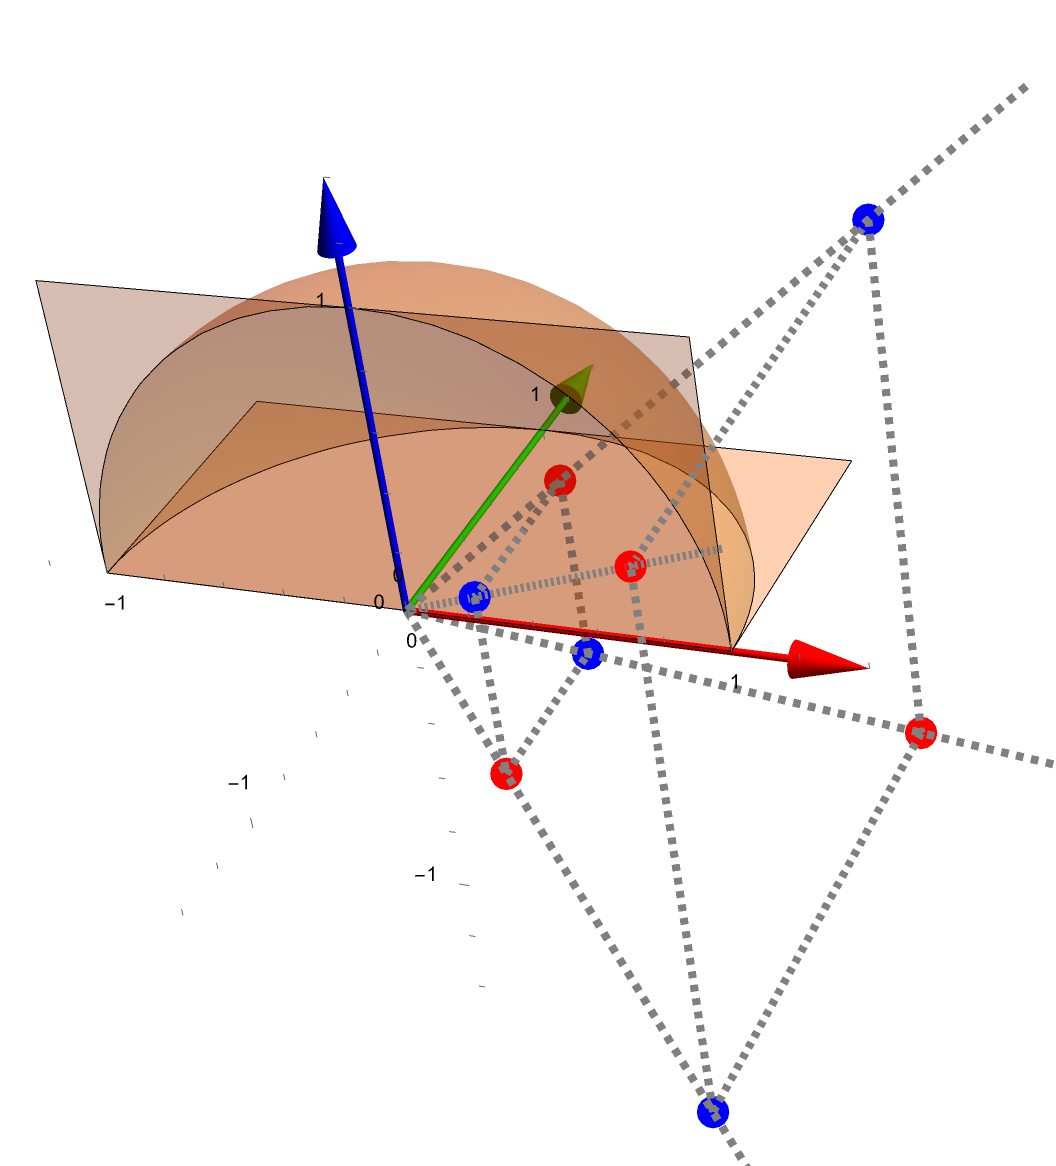
\includegraphics[width=0.75\textwidth]{images/hw_2_problem_1.png}
    \caption{Малюнок до задачі 2.1 (4). \textcolor{red}{\textbf{Червоним}} зображено позитивні заряди, \textcolor{blue}{\textbf{синім}} --- негативні. \textcolor{orange}{\textbf{Помаранчевим}} позначено границі області $\Omega$.}
    \label{fig:hw_2_problem_1}
\end{figure}
\pagebreak

Отже, тепер давайте аналітично зрозуміємо, що відбулось. Нехай ми маємо деяку точку $\mathbf{x} = (x_1, x_2, x_3) \in \Omega$. Тоді, ми можемо знайти 3 відображення цієї точки відносно площин $x_2=0$, $x_3=0$ та поверхні кулі $\|\mathbf{x}\|=R$. Ці відображення будуть мати координати:
\begin{align*}
    \mathbf{x}_1 &= (x_1, -x_2, x_3), \\
    \mathbf{x}_2 &= (x_1, x_2, -x_3), \\
    \mathbf{x}_3 &= \frac{R^2}{\|\mathbf{x}\|^2} \cdot \mathbf{x} = \left(\frac{R^2x_1}{x_1^2 + x_2^2 + x_3^2}, \frac{R^2x_2}{x_1^2 + x_2^2 + x_3^2}, \frac{R^2x_3}{x_1^2 + x_2^2 + x_3^2}\right).
\end{align*}

Далі, щоб компенсувати точки $\mathbf{x}_1$ та $\mathbf{x}_2$, нам потрібно ще одна точка:
\begin{align*}
    \mathbf{x}_4 &= (x_1, -x_2, -x_3)
\end{align*}

Таким чином, точки $(\mathbf{x}_1,\dots,\mathbf{x}_4)$ утворили квадрат. Далі точку $\mathbf{x}_3$ ми можемо так само віддзеркалити відносно площин $x_2=0$, $x_3=0$. Отримаємо:
\begin{align*}
    \mathbf{x}_5 = \left(\frac{R^2x_1}{x_1^2 + x_2^2 + x_3^2}, -\frac{R^2x_2}{x_1^2 + x_2^2 + x_3^2}, \frac{R^2x_3}{x_1^2 + x_2^2 + x_3^2}\right), \\
    \mathbf{x}_6 = \left(\frac{R^2x_1}{x_1^2 + x_2^2 + x_3^2}, \frac{R^2x_2}{x_1^2 + x_2^2 + x_3^2}, -\frac{R^2x_3}{x_1^2 + x_2^2 + x_3^2}\right),
\end{align*}

Далі, можна або відобразити $\mathbf{x}_5$ відносно площини $x_3=0$ або $\mathbf{x}_6$ відносно площини $x_2=0$. Так чи інакше, сьома і остання точка:
\begin{equation*}
    \mathbf{x}_7 = \left(\frac{R^2x_1}{x_1^2 + x_2^2 + x_3^2}, -\frac{R^2x_2}{x_1^2 + x_2^2 + x_3^2}, -\frac{R^2x_3}{x_1^2 + x_2^2 + x_3^2}\right).
\end{equation*}

Також, не забудемо виписати знаки зарядів. Нехай $q_j \in \{-1,1\}$ --- заряд точки $\mathbf{x}_j$. Отже, маємо:
\begin{align*}
    q_1 &= -1, & q_2 &= -1, & q_3 &= -1, & q_4 &= 1, & q_5 &= 1, & q_6 &= 1, & q_7 &= -1.
\end{align*}

Також, ми дещо оминули важливе питання: чому нам не потрібно далі відображати точки, скажімо, $\mathbf{x}_1$, $\mathbf{x}_2$ та $\mathbf{x}_3$ відносно поверхні кулі? Це тому що таке відображення дасть точки $\mathbf{x}_5$, $\mathbf{x}_6$ та $\mathbf{x}_7$, відповідно. Дійсно, розглянемо, наприклад, точку $\mathbf{x}_1$. Її відображення відносно поверхні кулі буде мати координати:
\begin{equation*}
    \mathbf{x}_1' = \frac{R^2}{\|\mathbf{x}_1\|} \cdot \mathbf{x}_1 = \left(\frac{R^2x_1}{x_1^2 + x_2^2 + x_3^2}, -\frac{R^2x_2}{x_1^2 + x_2^2 + x_3^2}, \frac{R^2x_3}{x_1^2 + x_2^2 + x_3^2}\right) = \mathbf{x}_5.
\end{equation*}

Аналогічно для $\mathbf{x}_2$ та $\mathbf{x}_3$. Таким чином, ми отримаємо точки $\mathbf{x}_5$, $\mathbf{x}_6$ та $\mathbf{x}_7$ ще раз. Отже, ми можемо зупинитися на цьому кроці. Запишемо остаточну функцію Гріна:
\begin{align*}
    G(\mathbf{x}, \boldsymbol{\xi}) &= \frac{1}{4\pi\|\mathbf{x} - \boldsymbol{\xi}\|} - \frac{1}{4\pi\|\mathbf{x}_1 - \boldsymbol{\xi}\|} - \frac{1}{4\pi\|\mathbf{x}_2 - \boldsymbol{\xi}\|} + \frac{1}{4\pi\|\mathbf{x}_4 - \boldsymbol{\xi}\|} \\&- \frac{R}{4\pi\|\mathbf{x}\|\|\mathbf{x}_3 - \boldsymbol{\xi}\|} + \frac{R}{4\pi\|\mathbf{x}\|\|\mathbf{x}_5 - \boldsymbol{\xi}\|} + \frac{R}{4\pi\|\mathbf{x}\|\|\mathbf{x}_6 - \boldsymbol{\xi}\|} - \frac{R}{4\pi\|\mathbf{x}\|\|\mathbf{x}_7 - \boldsymbol{\xi}\|} \\
\end{align*}

\subsection{Номер 2.5.}

\begin{problem}
    Розв'язати задачу для рівняння Лапласа $\Delta u = 0$ для області 
    \begin{equation*}
        \Omega = \{(x_1,x_2,x_3) \in \mathbb{R}^3: x_1 < 0, x_2 < 0\}    
    \end{equation*}
    з граничними умовами 
    \begin{equation*}
        u\Big|_{x_1=0}=\sin 3x_2 \sin x_3, \quad u\Big|_{x_2=0} = 0.
    \end{equation*}
\end{problem}

\textbf{Розв'язання.} Для початку скористаємося методом електростатичних зображень для побудуви функції Гріна $G(\mathbf{x}, \boldsymbol{\xi})$. Розглянемо малюнок нижче.

\begin{figure}[H]
    \centering
    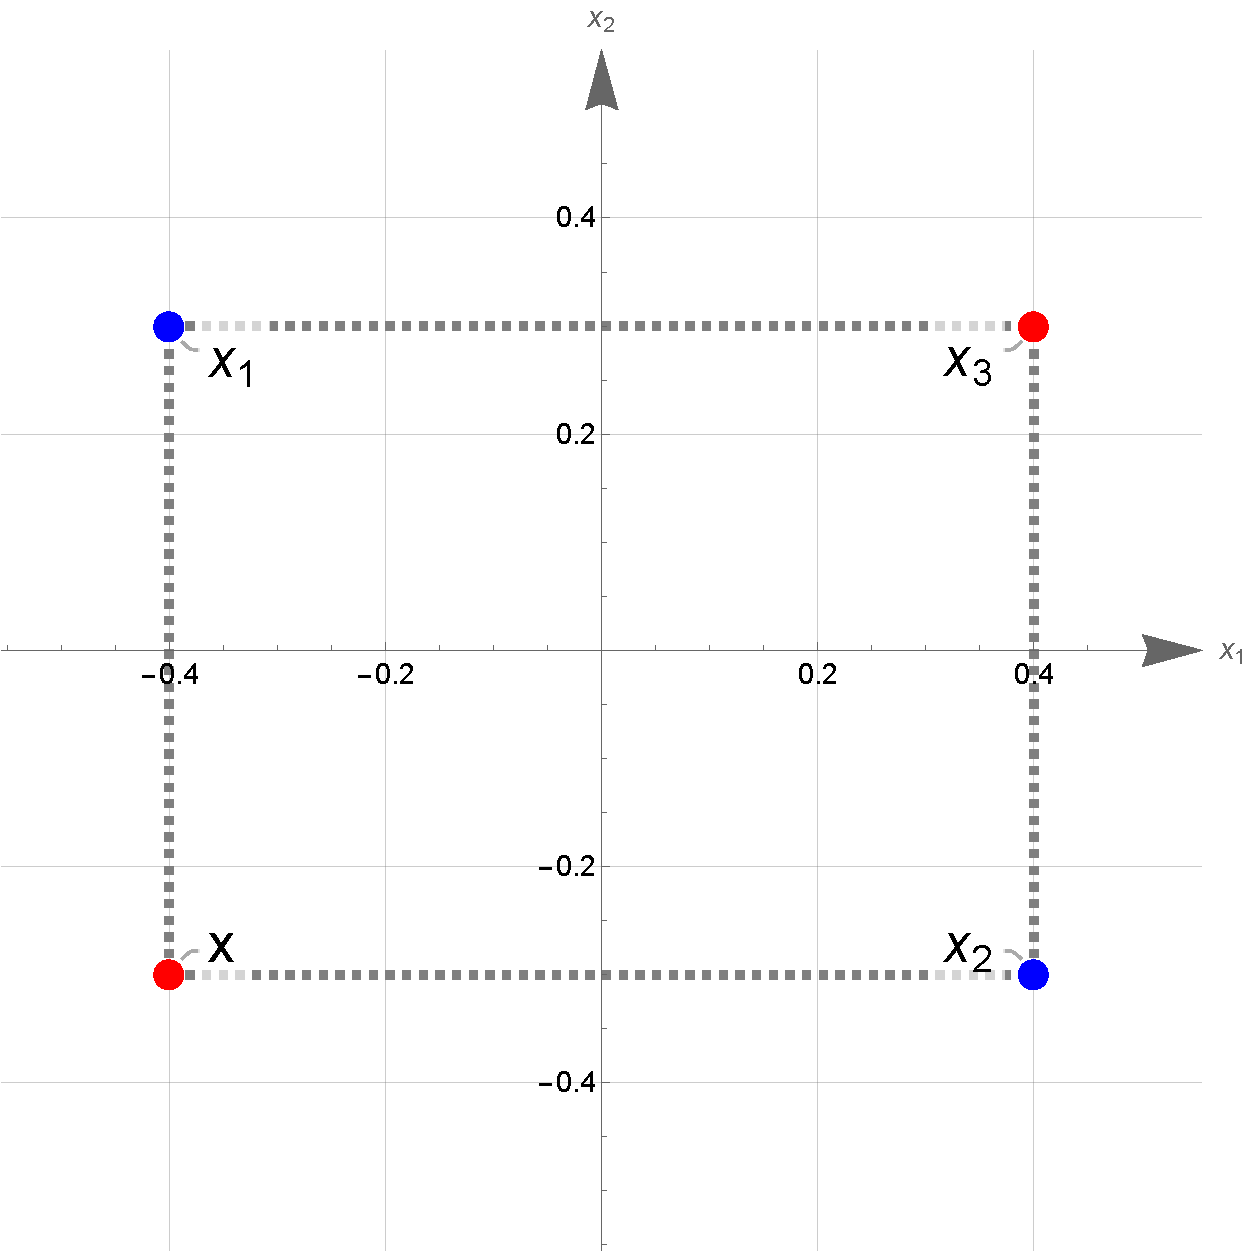
\includegraphics[width=0.65\textwidth]{images/hw_2_problem_2.pdf}
    \caption{Малюнок до задачі 2.5. Червоним зображено позитивні заряди, синім --- негативні. Малюнок у площині $Ox_1x_2$.}
    \label{fig:hw_2_problem_2}
\end{figure}

Тут маємо чотири точки:
\begin{align*}
    \mathbf{x} = (x_1,x_2,x_3), & \quad \text{знак $+$}, \\
    \mathbf{x}_1 = (x_1,-x_2,x_3), & \quad \text{знак $-$}, \\
    \mathbf{x}_2 = (-x_1,x_2,x_3), & \quad \text{знак $-$}, \\
    \mathbf{x}_3 = (-x_1,-x_2,x_3), & \quad \text{знак $+$}.
\end{align*}

В такому разі функція Гріна матиме вигляд:
\begin{align*}
    G(\mathbf{x}, \boldsymbol{\xi}) &= \frac{1}{4\pi\|\mathbf{x} - \boldsymbol{\xi}\|} - \frac{1}{4\pi\|\mathbf{x}_1 - \boldsymbol{\xi}\|} - \frac{1}{4\pi\|\mathbf{x}_2 - \boldsymbol{\xi}\|} + \frac{1}{4\pi\|\mathbf{x}_3 - \boldsymbol{\xi}\|}.
\end{align*}

На жаль, цей вираз доведеться розписати:
\begin{align*}
    G(\mathbf{x}, \boldsymbol{\xi}) &= \frac{1}{4\pi\sqrt{(x_1-\xi_1)^2 + (x_2-\xi_2)^2 + (x_3-\xi_3)^2}} - \frac{1}{4\pi\sqrt{(x_1-\xi_1)^2 + (x_2+\xi_2)^2 + (x_3-\xi_3)^2}} \\&- \frac{1}{4\pi\sqrt{(x_1+\xi_1)^2 + (x_2-\xi_2)^2 + (x_3-\xi_3)^2}} + \frac{1}{4\pi\sqrt{(x_1+\xi_1)^2 + (x_2+\xi_2)^2 + (x_3-\xi_3)^2}}.
\end{align*}

Далі скористаємось формулою репрезентації Гріна:
\begin{equation*}
    u(\mathbf{x}) = \iint_{\Omega} G(\mathbf{x}, \boldsymbol{\xi})f(\boldsymbol{\xi})d\boldsymbol{\xi} - \int_{\partial\Omega}\frac{\partial G(\mathbf{x}, \boldsymbol{\xi})}{\partial \boldsymbol{\nu}}\phi(\boldsymbol{\xi})dS_{\xi}
\end{equation*}

В нашому випадку $f(\boldsymbol{\xi})\equiv 0$, тому життя стало легше вдвічі. Також одразу помітимо, що в нас поверхня $\partial\Omega$ складається з двох частин: $x_1=0$ та $x_2=0$. Таким чином, ми можемо розбити інтеграл на два, позначивши першу частину як $\Omega_1$, а другу як $\Omega_2$:
\begin{equation*}
    u(\mathbf{x}) = -\int_{\Omega_1}\frac{\partial G(\mathbf{x}, \boldsymbol{\xi})}{\partial \boldsymbol{\nu}_1}\phi_1(\boldsymbol{\xi})dS_{\xi} - \int_{\Omega_2}\frac{\partial G(\mathbf{x}, \boldsymbol{\xi})}{\partial \boldsymbol{\nu}_2}\phi_2(\boldsymbol{\xi})dS_{\xi}.
\end{equation*}

Проте, за умовою $\phi_2(\boldsymbol{\xi}) \equiv 0$, тому залишається лише:
\begin{equation*}
    u(\mathbf{x}) = -\int_{\Omega_1}\frac{\partial G(\mathbf{x}, \boldsymbol{\xi})}{\partial \boldsymbol{\nu}_1}\phi_1(\boldsymbol{\xi})dS_{\xi}, \; \; \text{де} \; \;\phi_1(\boldsymbol{\xi}) = \sin 3\xi_2 \sin \xi_3, \; \boldsymbol{\nu}_1 = (1,0,0).
\end{equation*}

Залишається не дуже приємний етап: нам потрібно порахувати $(\partial G(\mathbf{x},\boldsymbol{\xi})/\partial \boldsymbol{\nu})\big|_{\xi_1=0}$. Отже маємо наступну часткову похідну:
\begin{align*}
    \frac{\partial G(\mathbf{x},\boldsymbol{\xi})}{\partial \boldsymbol{\nu}} = \frac{\partial G(\mathbf{x},\boldsymbol{\xi})}{\partial \xi_1} = \frac{x_1-\xi_1}{4\pi\left((x_1-\xi_1)^2 + (x_2-\xi_2)^2 + (x_3-\xi_3)^2\right)^{3/2}} \\- \frac{x_1-\xi_1}{4\pi\left((x_1-\xi_1)^2 + (x_2+\xi_2)^2 + (x_3-\xi_3)^2\right)^{3/2}} \\
    + \frac{x_1+\xi_1}{4\pi\left((x_1+\xi_1)^2 + (x_2-\xi_2)^2 + (x_3-\xi_3)^2\right)^{3/2}} \\ - \frac{x_1+\xi_1}{4\pi\left((x_1+\xi_1)^2 + (x_2+\xi_2)^2 + (x_3-\xi_3)^2\right)^{3/2}}.
\end{align*}

Отже, підставляємо умову на те, що $\xi_1=0$:
\begin{align*}
    \frac{\partial G(\mathbf{x},\boldsymbol{\xi})}{\partial \boldsymbol{\nu}}\Big|_{\xi_1=0} = \frac{x_1}{2\pi\left(x_1^2+(x_2-\xi_2)^2+(x_3-\xi_3)^2\right)^{3/2}} - \frac{x_1}{2\pi\left(x_1^2+(x_2+\xi_2)^2+(x_3-\xi_3)^2\right)}
\end{align*}

Тепер можемо підставити це у вираз для $u(\mathbf{x})$ та обчислити інтеграл. Отримаємо:
\begin{align*}
    u(\mathbf{x}) = -\int_{\Omega_1}\frac{\partial G(\mathbf{x}, \boldsymbol{\xi})}{\partial \boldsymbol{\nu}_1}\phi_1(\boldsymbol{\xi})dS_{\xi} &= -\int_{-\infty}^{\infty}\int_{-\infty}^{0}\frac{x_1\sin 3\xi_2 \sin \xi_3}{2\pi\left(x_1^2+(x_2-\xi_2)^2+(x_3-\xi_3)^2\right)^{3/2}} d\xi_2 d\xi_3 \\&+ \int_{-\infty}^{\infty}\int_{-\infty}^{0}\frac{x_1\sin 3\xi_2 \sin \xi_3}{2\pi\left(x_1^2+(x_2+\xi_2)^2+(x_3-\xi_3)^2\right)^{3/2}} d\xi_2 d\xi_3.
\end{align*}

Далі залишається лише шаманити:
\begin{align*}
    u(\mathbf{x}) = \frac{x_1}{2\pi}\int_{-\infty}^{+\infty}\Bigg(-\sin\xi_3\int_{-\infty}^0 \frac{\sin 3\xi_2d\xi_2}{\left(x_1^2+(x_2-\xi_2)^2+(x_3-\xi_3)^2\right)^{3/2}} \\+ \sin\xi_3 \int_{-\infty}^0 \frac{\sin 3\xi_2d\xi_2}{\left(x_1^2+(x_2+\xi_2)^2+(x_3-\xi_3)^2\right)^{3/2}} \Bigg)d\xi_3
\end{align*}

Тепер пропонується наступне: у першому внутрішньому інтегралі зробити наступну заміну: $\xi_2 \mapsto -\xi_2$. Тоді межі інтегрування зміняться на від $+\infty$ до $0$. В такому разі маємо:
\begin{align*}
    u(\mathbf{x}) = \frac{x_1}{2\pi}\int_{-\infty}^{+\infty}\Bigg(-\sin\xi_3\int_{+\infty}^0 \frac{\sin (-3\xi_2)d(-\xi_2)}{\left(x_1^2+(x_2+\xi_2)^2+(x_3-\xi_3)^2\right)^{3/2}} \\+ \sin\xi_3 \int_{-\infty}^0 \frac{\sin 3\xi_2d\xi_2}{\left(x_1^2+(x_2+\xi_2)^2+(x_3-\xi_3)^2\right)^{3/2}} \Bigg)d\xi_3
\end{align*}

Мінуси всередині інтегралу скорочуються, а мінус перед інтегралом приберемо, змінивши межі інтегрування. Отже, маємо:
\begin{align*}
    u(\mathbf{x}) &= \frac{x_1}{2\pi}\int_{-\infty}^{+\infty}\Bigg(\sin\xi_3\int_{0}^{+\infty} \frac{\sin 3\xi_2d\xi_2}{\left(x_1^2+(x_2+\xi_2)^2+(x_3-\xi_3)^2\right)^{3/2}} \\&+ \sin\xi_3 \int_{-\infty}^0 \frac{\sin 3\xi_2d\xi_2}{\left(x_1^2+(x_2+\xi_2)^2+(x_3-\xi_3)^2\right)^{3/2}} \Bigg)d\xi_3 \\
    &= \frac{x_1}{2\pi}\int_{-\infty}^{+\infty}\left(\sin\xi_3\int_{-\infty}^{+\infty}\frac{\sin 3\xi_2d\xi_2}{\left(x_1^2+(x_2+\xi_2)^2+(x_3-\xi_3)^2\right)^{3/2}}\right)d\xi_3 \\
    &= \frac{x_1}{2\pi}\int_{-\infty}^{+\infty}\int_{-\infty}^{+\infty}\frac{\sin\xi_3\sin 3\xi_2d\xi_2d\xi_3}{\left(x_1^2+(x_2+\xi_2)^2+(x_3-\xi_3)^2\right)^{3/2}}
\end{align*}

Тепер зробимо заміну змінних $\eta_2 := x_2+\xi_2$, $\eta_3 := \xi_3-x_3$. Тоді маємо:
\begin{align*}
    u(\mathbf{x}) &= \frac{x_1}{2\pi}\int_{-\infty}^{+\infty}\int_{-\infty}^{+\infty}\frac{\sin(\eta_3+x_3)\sin(3\eta_2-3x_2)d\eta_2d\eta_3}{\left(x_1^2+\eta_2^2+\eta_3^2\right)^{3/2}}
\end{align*}

Тепер помітимо наступний факт:
\begin{align*}
    \sin(\eta_3+x_3)\sin(3\eta_2-3x_2) &= (\sin\eta_3\cos x_3+\cos\eta_3 \sin x_3)(\sin 3\eta_2 \cos 3x_2 - \cos 3\eta_2 \sin 3x_2) \\
    &= \sin\eta_3\sin 3\eta_2 \cos x_3 \cos 3x_2 - \sin\eta_3\cos x_3 \cos 3\eta_2\sin 3x_2\\
    &+ \cos\eta_3 \sin x_3\sin 3\eta_2 \cos 3x_2 - \cos\eta_3 \sin x_3\cos 3\eta_2 \sin 3x_2
\end{align*}

Помітимо, що якщо ми розпишемо інтеграл на чотири окремі інтеграли, то усі, окрім четвертого, будуть нульовими через непарність функції $\sin$. Таким чином, маємо:
\begin{align*}
    u(\mathbf{x}) &= -\frac{x_1\sin x_3 \sin 3x_2}{2\pi}\int_{-\infty}^{+\infty}\int_{-\infty}^{+\infty}\frac{\cos\eta_3\cos 3\eta_2 d\eta_2d\eta_3}{\left(x_1^2+\eta_2^2+\eta_3^2\right)^{3/2}}
\end{align*}

Отже, позначимо:
\begin{equation*}
    \psi(x_1) = -\frac{x_1}{2\pi}\int_{-\infty}^{+\infty}\int_{-\infty}^{+\infty}\frac{\cos\eta_3\cos 3\eta_2 d\eta_2d\eta_3}{\left(x_1^2+\eta_2^2+\eta_3^2\right)^{3/2}}
\end{equation*}

Звичайно, обрахувати цей інтеграл аналітично дуже складно, тому ми знайдемо цю функцію іншим способом. Маємо, що наш розв'язок:
\begin{equation*}
    u(x_1,x_2,x_3) = \sin x_3 \sin 3x_2 \cdot \psi(x_1).
\end{equation*}

Отже, знайдемо Лапласіан цієї функції:
\begin{align*}
    \Delta u(x_1,x_2,x_3) &= \frac{\partial^2 u}{\partial x_1^2} + \frac{\partial^2 u}{\partial x_2^2} + \frac{\partial^2 u}{\partial x_3^2} \\
    &= \sin x_3 \sin 3x_2 \cdot \psi''(x_1) - 9\sin x_3 \sin 3x_2 \cdot \psi(x_1) - \sin x_3 \sin 3x_2 \cdot \psi(x_1) \\
    &= \sin x_3 \sin 3x_2 \cdot \psi''(x_1) - 10\sin x_3 \sin 3x_2 \cdot \psi(x_1) \\
    &= \sin x_3 \sin 3x_2(\psi''(x_1) - 10\psi(x_1)) = 0
\end{align*}

Отже маємо диференціальне рівняння відносно $\psi(x_1)$:
\begin{equation*}
    \psi''(x_1) = 10\psi(x_1)
\end{equation*}

Як відомо, розв'язок такого рівняння $\psi(x_1) = C_1e^{\sqrt{10}x_1} + C_2e^{-\sqrt{10}x_1}$. Оскільки розв'язок має бути обмеженим, причому для $x_1<0$, то $C_2=0$. Константу $C_1$ знайдемо з граничної умови: $u(0,x_2,x_3)=\sin x_3 \sin 3x_2 \cdot \psi(0) = \sin x_3 \sin 3x_2$, звідки $\psi(0)=1$. Отже, $C_1=1$, тому остаточно:
\begin{equation*}
    \boxed{u(x_1,x_2,x_3) = \sin x_3 \sin 3x_2 e^{\sqrt{10}x_1}}.
\end{equation*}

\pagebreak

\subsection{Номер 2.6.}

\begin{problem}
    Довести додатність функції Гріна задачі Діріхле для оператора Лапласа в обмеженій області. 
    
    \textit{Підказка.} Використати принцип максимуму.
\end{problem}

\textbf{Розв'язання.} Отже, нехай перед нами задача Діріхле для оператора Лапласа:
\begin{align*}
    &\Delta u(\mathbf{x}) = 0, \quad \mathbf{x} \in \Omega \subset \mathbb{R}^m, \\
    &u(\mathbf{x}) = \phi(\mathbf{x}) \quad \mathbf{x} \in \partial\Omega,
\end{align*}

де $\phi: \partial\Omega \to \mathbb{R}$ --- це задана функція.

Як було доведено на лекції, розв'язок цієї задачі можна записати у вигляді:
\begin{equation*}
    u(\mathbf{x}) = -\int_{\partial\Omega} \frac{\partial G(\mathbf{x},\boldsymbol{\xi})}{\partial\boldsymbol{\nu}}\phi(\boldsymbol{\xi})d_{\xi}S,
\end{equation*}

де $G(\mathbf{x},\boldsymbol{\xi})$ --- наша функція Гріна. Потрібно довести, що $G(\mathbf{x}_0, \boldsymbol{\xi}) \succ 0$ для $\mathbf{x}_0 \in \text{int}(\Omega)$. Для початку згадаємо з означення, що на границі ми маємо мати:
\begin{equation*}
    G(\mathbf{x}, \boldsymbol{\xi}) = 0, \quad \forall\boldsymbol{\xi} \in \partial\Omega.
\end{equation*}

Цей факт спонукає застосувати принцип максимуму. Нагадаємо його.
\begin{theorem}[Принцип максимуму]
    Якщо $u(\mathbf{x}) \in \mathcal{C}(\overline{\Omega})$ --- гармонічна функція в обмеженій області $\Omega$, то вона приймає свої $\max$ та $\min$ значення на границі $\partial\Omega$.
\end{theorem}

Наша функція $G$ є гармонічною за $\boldsymbol{\xi}$ ($\mathbf{x}_0$ є фіксованим) в $\Omega \setminus B_{\varepsilon}(\mathbf{x}_0)$ для деякого малого $\varepsilon > 0$, а тому застосувавши цю теорему ми знаємо, що $G$ досягає свого мінімума або максимума на $\partial\Omega$, тобто нуля. Більш того, оскільки границі у нас по суті дві, то інший екстремум буде досягатися на $\partial B_{\varepsilon}(\mathbf{x}_0)$. Залишається дізнатися де максимум, де мінімум, і які значення вони мають.

З означення можна пригадати, що $G(\mathbf{x}_0, \boldsymbol{\xi}) \xrightarrow[\boldsymbol{\xi} \to \mathbf{x}_0]{} +\infty$, що означає
\begin{equation*}
    (\forall \rho > 0) \; (\exists \varepsilon > 0): \{G(\mathbf{x}_0, \boldsymbol{\xi}) > \rho\} \; \text{для $\boldsymbol{\xi} \in \partial B_{\varepsilon}(\mathbf{x}_0)$}
\end{equation*}

Отже можна покласти будь-яке $\rho > 0$, зафіксувати відповідне $\varepsilon$ і в нас буде принаймі одне додатнє значення на границі $\partial B_{\varepsilon}(\mathbf{x}_0)$. Таким чином, на одній межі $\partial\Omega$ в нас $0$, а на іншій $\partial B_{\varepsilon}$ --- додатне значення. Отже, функція Гріна є додатно визначеною в усій множині $\text{int}(\Omega) \setminus B_{\varepsilon}(\mathbf{x}_0)$. Взявши перехід $\varepsilon \to 0$, ми узагальнимо цей результат на всю область $\text{int}(\Omega)$. Отже, функція Гріна є додатно визначеною в усій області $\text{int}(\Omega)$.

\end{document}